\documentclass[a4paper,review,12pt]{elsarticle}

\usepackage[utf8]{inputenc}
\usepackage[T5]{fontenc}
\usepackage{booktabs}
\usepackage{tabularx}
\usepackage{array}
\usepackage{graphicx}
\usepackage{float}
\usepackage{microtype}
\usepackage{xurl}
\usepackage[hidelinks]{hyperref}

\newcommand{\method}{PACE-Seg}
\newcommand{\miou}{mIoU}
\setlength{\emergencystretch}{2em}
\renewcommand{\thefigure}{S\arabic{figure}}
\renewcommand{\theHfigure}{S\arabic{figure}}
\renewcommand{\thetable}{S\arabic{table}}
\renewcommand{\theHtable}{S\arabic{table}}

\begin{document}

\begin{frontmatter}
\title{Supplementary Material for PACE-Seg: Hardware-Cost-Conditioned Elastic Semantic Segmentation with Calibrated Risk Routing for Edge Accelerators}
\author{D\~{u}ng Nguy\~{\^{e}}n}
\begin{abstract}
This supplement records the detailed experimental protocol, checkpoint and runtime provenance, secondary fake-quant study, complete-route expansion, condition-level routing results, and extended qualitative evidence for the PACE-Seg manuscript. It does not introduce new headline claims or independent evaluation samples.
\end{abstract}
\end{frontmatter}

\section{Evidence scope}

The main manuscript reports the three primary findings: measured hardware cost is necessary for budget feasibility, shared elastic training preserves matched-capacity quality, and candidate-specific hard-budget routing improves the descriptive quality--cost trade-off. This supplement preserves implementation and audit details that are necessary for reproducibility but not for following that central argument. The 120 routing cells remain correlated evaluations, and E1/E3 reuse segmentation predictions.

\section{Training and checkpoint provenance}

Elastic training uses the sandwich rule: each step evaluates the smallest and largest levels and one randomly selected intermediate level. The largest level receives supervised segmentation loss; smaller levels receive supervised and in-place distillation terms; and a boundary auxiliary term emphasizes semantic transitions. Training uses 100,000 optimization steps, batch size 8, AdamW with weight decay $10^{-4}$, initial learning rate $3\times10^{-4}$, cosine decay, 500 warm-up steps, and gradient clipping at 5.0. The data stream combines Cityscapes and ACDC with random scale/crop/pad, horizontal flip, and color jitter.

The near-parity comparison uses three reported supernet runs and three augmented Fast-SCNN runs. Router analysis uses the three separately trained checkpoints in Table~\ref{tab:provenance}. Initialization-parent identifiers and immutable full training manifests remain unavailable, so Runs A--C are not described as a perfectly controlled identical-configuration seed study.

\begin{table}[H]
\centering
\caption{Training-checkpoint provenance used by router analysis. Hashes are abbreviated; full SHA-256 values are retained in the evidence manifest and canonical replay manifest.}
\label{tab:provenance}
\small
\begin{tabularx}{\textwidth}{@{}lXlll@{}}
\toprule
Run & Training record & Step & Checkpoint SHA & Config hash \\
\midrule
A & Augmentation-labelled & 100,000 & \texttt{a2444156} & \texttt{6d1274f40e43} \\
B & Earlier unlabelled & 100,000 & \texttt{00da283c} & \texttt{837cf981427a} \\
C & Augmentation-labelled & 100,000 & \texttt{275dfcbf} & \texttt{ac52eabac3de} \\
\bottomrule
\end{tabularx}
\end{table}

Fixed-architecture comparisons cover Fast-SCNN, BiSeNetV2, SegFormer-B0, DDRNet-23-slim, and MobileNetV3/DeepLabV3. Fast-SCNN is the parameter-matched comparator for the large elastic level. Routing references include static candidates, raw entropy, rank-based policy A, latency-spacing policy B, candidate-specific policy C without a hard budget, configured and pooled variants of constrained policy D, and a non-deployable oracle.

\section{Hardware, compiler, and latency protocol}

Table~\ref{tab:hardware} records the toolchain-specific deployment environments. TensorRT measurements use GPU FP16. Hailo candidates are compiled from ONNX through Hailo's Dataflow Compiler to HEF. Compiler smoke tests establish that all four static candidates execute on the primary TensorRT GPU and Hailo paths. DLA is excluded from headline analysis because decoder execution falls back to the GPU.

\begin{table}[H]
\centering
\caption{Hardware and compiler stacks used for candidate-latency measurement.}
\label{tab:hardware}
\small
\begin{tabularx}{\textwidth}{@{}llX@{}}
\toprule
ID & Hardware & Runtime and system versions \\
\midrule
E1 & Raspberry Pi 5 + Hailo-8 M.2 & HailoRT 4.23.0; HEFs from Dataflow Compiler 3.34.0 and Model Zoo 2.19.0 \\
E2 & Jetson Xavier NX & L4T R35.4.1; CUDA 11.4.19; cuDNN 8.6.0.166; TensorRT 8.5.2.2 \\
E3 & Jetson AGX Xavier & L4T R35.6.4; CUDA 11.4.19; TensorRT 8.5.2.2 \\
E5 & Jetson Orin Nano Super & L4T R36.5.0; CUDA 12.6.68; cuDNN 9.3.0; TensorRT 10.3.0.30 \\
\bottomrule
\end{tabularx}
\end{table}

Candidate-only latency uses batch size one, warm-up, three independent benchmark runs for the lookup table, and bootstrap intervals. Complete warm-route costs are measured on E1 and E3. On E3, all four TensorRT contexts are resident and timing includes tiny inference, device-resident entropy, policy evaluation, dispatch, and additional candidate inference. On E1, timing includes mandatory network-group activation and deactivation, tiny inference, host entropy, policy evaluation, and additional candidate inference. Each route class uses 50 warm-up iterations and at least 500 timed iterations. Backend-specific cold-start measurements are excluded because the runtimes impose different reload semantics.

The timing harnesses use compiled graphs with the correct post-rescale architecture but do not execute the trained weights that produce the accuracy caches. The study combines measured route latency with cached trained-model predictions in offline per-image replay. A production-path audit on 40 TensorRT outputs measures a maximum risk-score deviation of $7.15\times10^{-7}$ nats from the PyTorch reference, below the prespecified $10^{-4}$ tolerance. Energy is excluded because no calibrated external power meter was available.

\section{Router unit of analysis and leakage safeguards}

Segmentation quality is dataset-level \miou{}. Router calibration targets per-image pixel error, while routed quality is recomputed by accumulating confusion matrices from selected candidates and calculating \miou{} once over the routed held-out set. The reporting unit is an operating cell defined by checkpoint, backend cost table, dataset split, and budget. Cells reuse images, predictions, thresholds, and candidate sets, so descriptive counts and macro averages are reported without cell-level significance tests.

A fair A-versus-D cell is one in which A has zero held-out per-image budget violations at its fit-selected operating point. A cell is violating when at least one held-out image exceeds its budget. Fair-cell quality counts are paired with full-grid violation counts. D's zero violating-cell count is partly structural because D removes candidates above budget.

Every candidate is evaluated once per image and its prediction is cached. The probe feature is mean softmax entropy over all output pixels in both fitting and deployment. Condition-specific calibrators use only fit-half probe scores and candidate errors; pooled calibration combines only fit halves across the five splits. Five risk targets are the 10th, 25th, 50th, 75th, and 90th percentiles of fit-half observed error, macro-aggregated across splits. One grid is generated per checkpoint and reused across E1 and E3 cost tables.

For each budget and policy, the representative risk target is selected from fit-half statistics by maximizing fit-half \miou{} among points whose mean cost satisfies the budget, with lower cost as the tie-break. Held-out outcomes are read only after selection. Held-out labels do not fit calibrators, define thresholds, or select operating points; they reconstruct final routed \miou{} and budget violations. Historical masked-fit artifacts remain available for audit but are not used for the RQ3 headline.

\section{Secondary fake-quant study}

QAT replaces each convolution with per-tensor symmetric 8-bit fake quantization of its input activation and active weight tensor using a straight-through estimator. Dynamic mode derives activation scale from every call. Calibrated mode freezes one activation range per layer after a 200-image calibration pass spanning clean and adverse conditions. The maximum observer retains the largest activation observed, while the EMA-percentile observer tracks the 99.9th percentile of absolute activation with momentum 0.9.

One calibration buffer belongs to each shared slimmable layer and aggregates calls from all elasticity levels; the implementation does not maintain a separate frozen activation scale for each level. Each QAT run fine-tunes 10,000 steps from an FP32 checkpoint at learning rate $3\times10^{-5}$. These are simulated fake-quant results, not integer-kernel or compiled INT8 measurements.

Dynamic fake quantization of the shared large level loses 1.66, 2.54, and 1.39 \miou{} points in the worst condition of Runs A--C. EMA-percentile calibration produces the bounds in Table~\ref{tab:qat}. The worst large-level degradation improves from 2.54 to 1.38 points, but mean effects are not uniformly positive and the data do not directly measure activation outliers.

\begin{table}[H]
\centering
\caption{Absolute worst-condition \miou{} degradation under shared-supernet EMA-percentile fake-quant QAT.}
\label{tab:qat}
\begin{tabular}{@{}lrrrr@{}}
\toprule
Training run & tiny & small & medium & large \\
\midrule
Run A & 0.32 & 0.97 & 0.51 & 0.97 \\
Run B & 0.69 & 0.33 & 0.49 & 1.38 \\
Run C & 0.36 & 0.33 & 0.56 & 0.86 \\
\bottomrule
\end{tabular}
\end{table}

\section{Expanded qualitative error gallery}

Figure~\ref{fig:qualitative-failure} combines the five deterministic median-error split representatives with the predetermined highest-error Run A ACDC night case. It illustrates error structure and does not estimate a failure rate.

\clearpage
\begin{figure}[H]
\centering
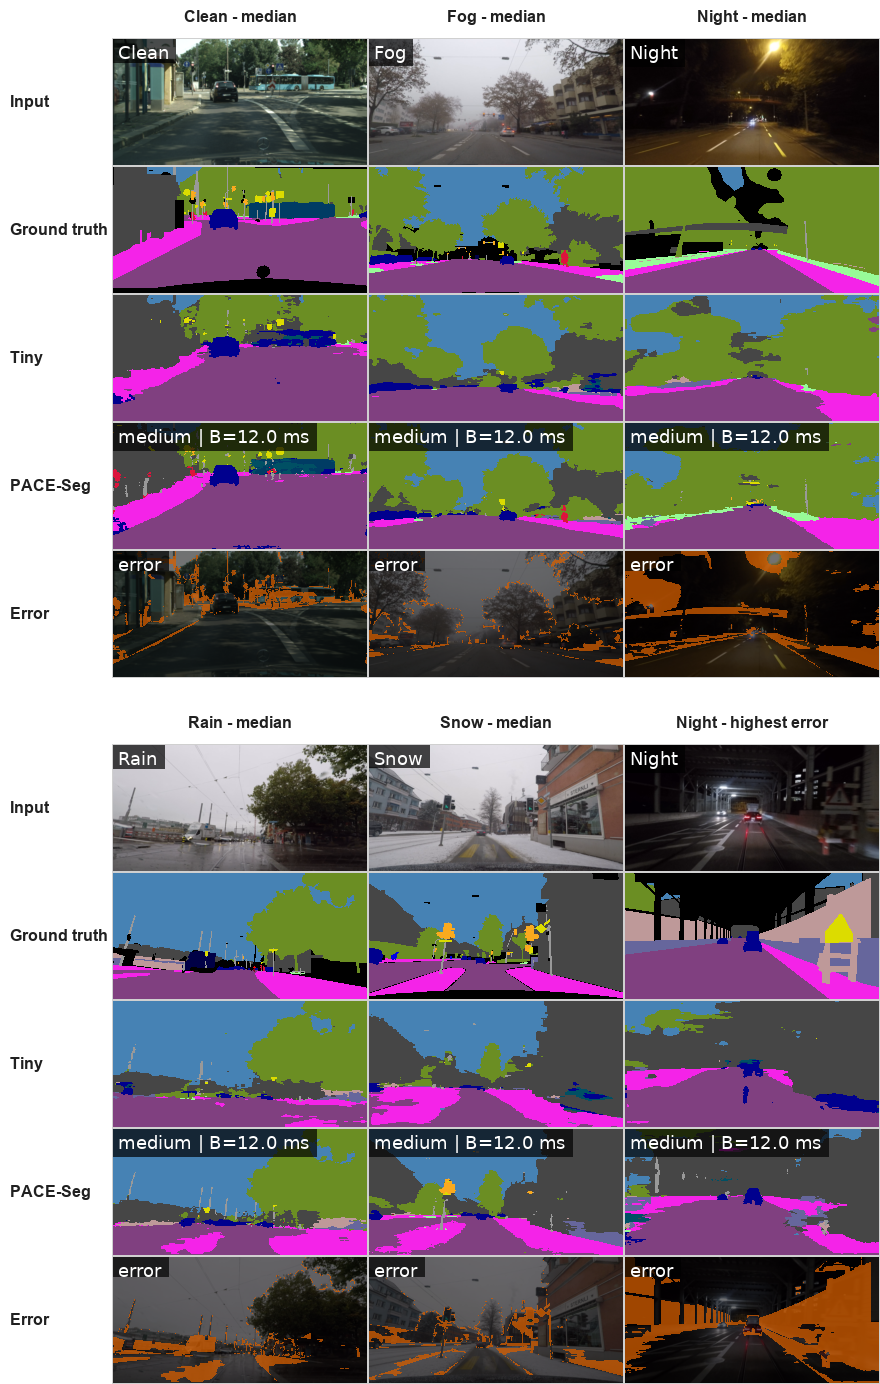
\includegraphics[height=0.75\textheight,keepaspectratio]{figures/figS1_failure_gallery.png}
\caption{Expanded qualitative error gallery. The six audited examples comprise the five deterministic median-error split representatives and the predetermined highest-error Run A ACDC night case. Each example compares input, ground truth, tiny, configured policy-D output, and output error; orange marks disagreement with ground truth.}
\label{fig:qualitative-failure}
\end{figure}

\section{Candidate-only versus complete route cost}

Figure~\ref{fig:route-cost-expansion} compares isolated candidate latency with complete warm-route latency. The gap is largest for low-capacity Hailo-8 routes because activation and host-side work dominate their short isolated inference time. The bars compare two measured totals and are not a component decomposition.

\begin{figure}[H]
\centering
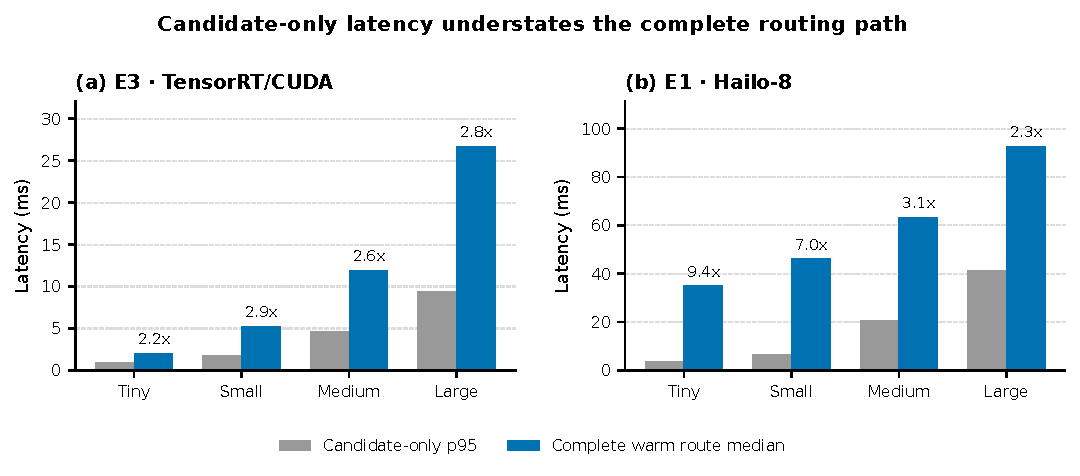
\includegraphics[width=\linewidth]{figures/figS2_route_cost_expansion.pdf}
\caption{Candidate-only p95 latency versus measured complete warm-route median. The complete route includes the tiny probe, risk computation, policy evaluation, backend dispatch or activation, and any additional candidate inference. Ratios above the bars quantify expansion relative to isolated candidate p95.}
\label{fig:route-cost-expansion}
\end{figure}

\section{Additional audited qualitative views}

Figures~\ref{fig:additional-qualitative} and~\ref{fig:local-crops} reorganize the same six audited examples used in Fig.~\ref{fig:qualitative-failure}. They do not introduce condition-specific easy/hard samples or additional evaluation observations.

\begin{figure}[H]
\centering
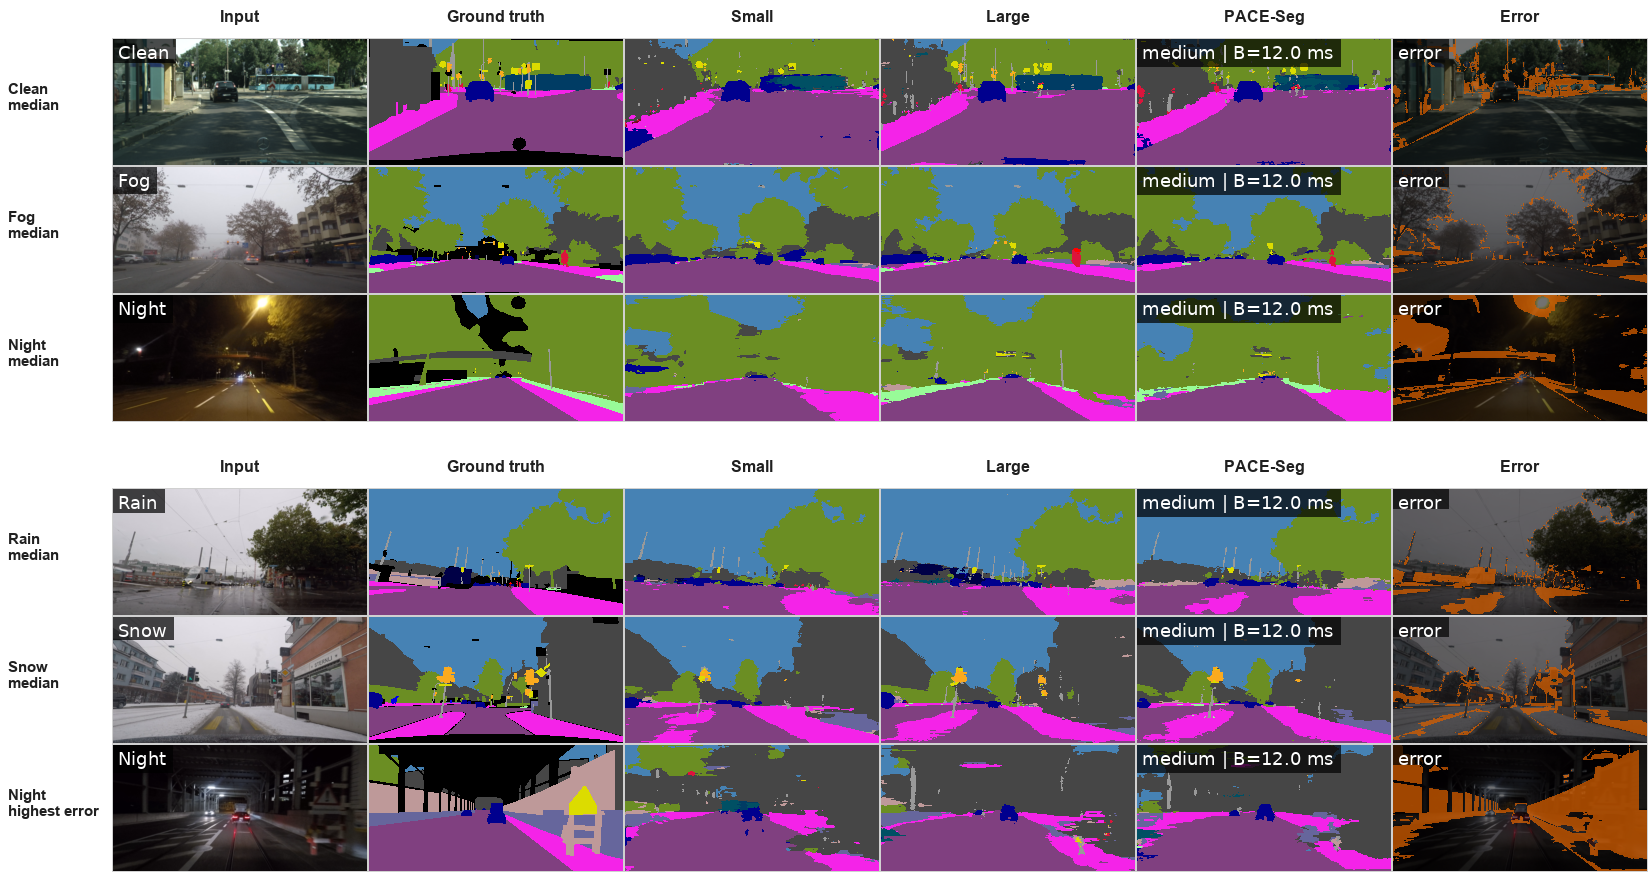
\includegraphics[width=\linewidth]{figures/figS3_additional_qualitative.png}
\caption{Additional full-frame comparison of the six audited examples. Columns show input, ground truth, small, large, configured policy-D output, and selected-output error. This is not an easy-versus-hard sampling study.}
\label{fig:additional-qualitative}
\end{figure}

\begin{figure}[H]
\centering
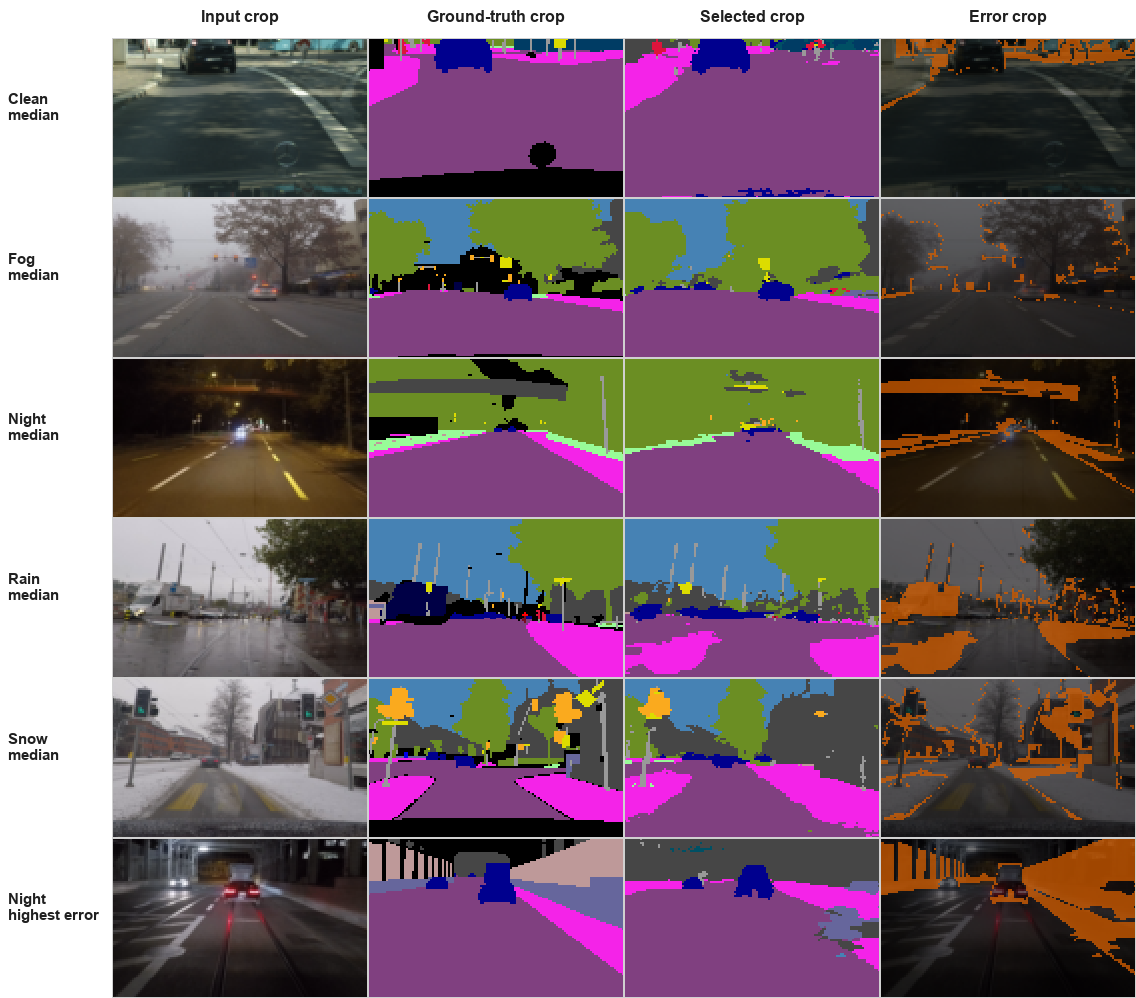
\includegraphics[width=\linewidth]{figures/figS4_local_crops.png}
\caption{Local error crops from the same six audited examples. Every crop uses the fixed normalized window $x=[0.25,0.75]$ and $y=[0.36,1.00]$, rather than image-specific manual framing.}
\label{fig:local-crops}
\end{figure}

\section{Condition-level routing summary}

Table~\ref{tab:router-condition} disaggregates the canonical deployment-matched comparison by visual condition. Counts pool three training runs and two backend cost tables, so cells remain correlated and E1/E3 share segmentation predictions. Fair cells are those in which policy A has zero held-out budget violations.

\begin{table}[H]
\centering
\caption{Condition-level configured and pooled D comparisons against policy A. W/T/L and mean $\Delta$ use fair cells; violation counts use all 24 cells per condition. Configured and pooled D each have zero violations.}
\label{tab:router-condition}
\scriptsize
\setlength{\tabcolsep}{3.0pt}
\resizebox{\textwidth}{!}{%
\begin{tabular}{@{}lrrrrrrr@{}}
\toprule
Condition & Fair & Config. W/T/L & Config. $\Delta$ & Pooled W/T/L & Pooled $\Delta$ & A viol. & D viol. \\
\midrule
Cityscapes & 7/24 & 7/0/0 & +0.0610 & 7/0/0 & +0.0612 & 17/24 & 0/24 \\
ACDC/Fog & 20/24 & 14/4/2 & +0.0373 & 16/4/0 & +0.0392 & 4/24 & 0/24 \\
ACDC/Night & 11/24 & 11/0/0 & +0.0125 & 11/0/0 & +0.0125 & 13/24 & 0/24 \\
ACDC/Rain & 24/24 & 12/10/2 & +0.0248 & 14/10/0 & +0.0271 & 0/24 & 0/24 \\
ACDC/Snow & 12/24 & 12/0/0 & +0.0160 & 10/0/2 & +0.0157 & 12/24 & 0/24 \\
\bottomrule
\end{tabular}
%
}
\end{table}

\section{Evidence locations}

The canonical routing directory is \path{reports/router_deployment_matched_20260929/}. Its manifest records code commit, checkpoint and configuration hashes, command chain, and output hashes. The submission evidence manifest maps every figure and numerical claim to machine-readable artifacts. Raw Cityscapes and ACDC data and training checkpoints are not redistributed because of dataset licensing and storage constraints.

\end{document}
